\documentclass[11pt,a4paper,bibliography=totocnumbered]{scrartcl}
\usepackage[utf8]{inputenc}
\usepackage[british]{babel}
%\usepackage{amsmath}
%\usepackage{amsfonts}
%\usepackage{amssymb}
\usepackage[footsepline]{scrlayer-scrpage}
\usepackage{tabu}
\usepackage{placeins}
%\usepackage{longtable}
\usepackage{multirow}
\usepackage{setspace}
%\usepackage{graphicx}
%\usepackage{pgfplots}
\usepackage{hyperref}
\usepackage{url}
\usepackage{titling}
\usepackage[backend=biber,sorting=none]{biblatex}
\usepackage{csquotes}
\usepackage{pdfpages}
\usepackage{epstopdf}
\usepackage{graphicx}
\usepackage{subfig}
\usepackage{array}
%\usepackage{enumitem}
\usepackage[backgroundcolor=lightgray]{todonotes}

%\pgfplotsset{width=12cm,height=6cm,compat=1.11}

% Constants
\def\mytitle{Tomcat Native 2}
\def\myauthor{Jocelyn Thode and Simon Brulhart}
\def\theclient{Red Hat}

\pagestyle{scrheadings}

\ihead{\mytitle}
\chead{}
\cfoot{}
\ifoot{Initial plan}
\ofoot{\thepage}

\posttitle{\end{center}\begin{center}\LARGE Final Report\end{center}}

\author{\myauthor\\ \href{mailto:jocelyn.thode@unifr.ch}{jocelyn.thode@unifr.ch} \\ \href{mailto:simon.brulhart@unifr.ch}{simon.brulhart@unifr.ch}}
\title{\huge \textbf{\mytitle}}

\bibliography{final_report}

\begin{document}

\graphicspath{{figures/}}

\begin{titlingpage}

\maketitle

\begin{abstract}
\mytitle{} is a project mandated by Red Hat. It aims at providing a JNI wrapper for OpenSSL for use in both Undertow and Tomcat. This project is the practical part of the R\&D Workshop course given at the University of Neuchâtel as part of the Joint Master in Computer Science.
\end{abstract}

\begin{figure}[b]
\centering
\subfloat{
\includegraphics[height=1.8cm]{unine.eps}}
\qquad
\subfloat{
\includegraphics[height=1.5cm]{jmcs.png}}
\qquad
\subfloat{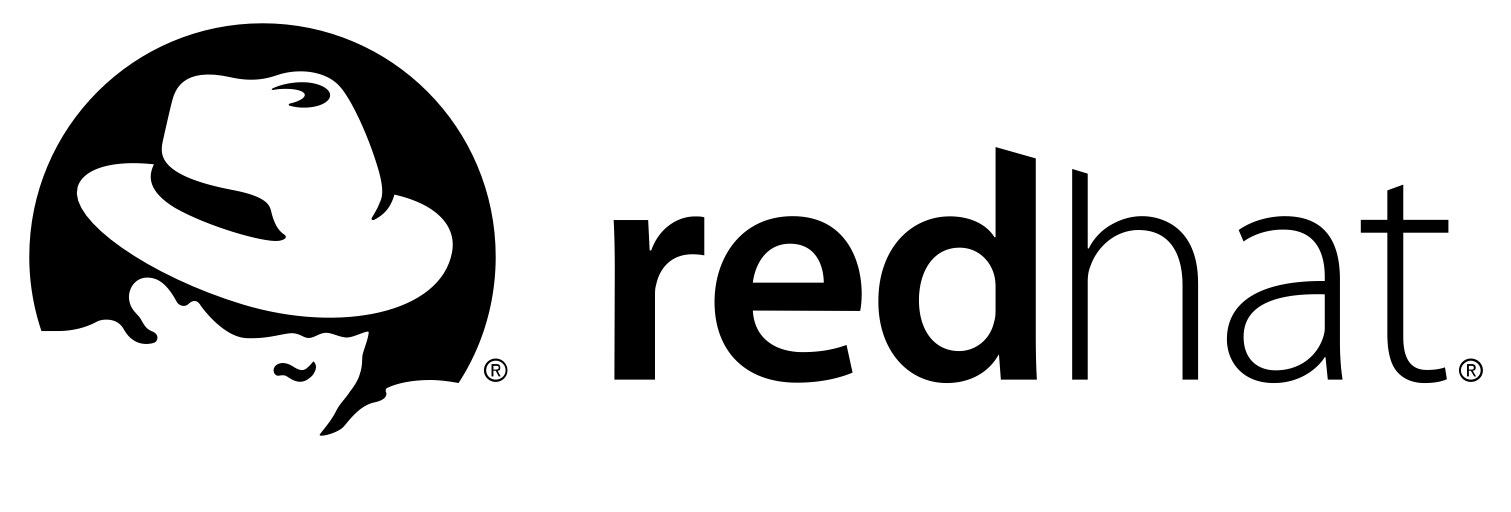
\includegraphics[height=1.6cm]{redhat-logo.png}}
\end{figure}

\end{titlingpage}

\pagebreak

\setcounter{tocdepth}{2}
\tableofcontents
\listoffigures

\pagebreak

\section{Project description}

\subsection{Project context}
For this project we are working with \theclient{} which is a multinational software company that provides open-source software and technical support to enterprises\autocite{redhat}.
At the moment, Tomcat\autocite{tomcat} and Undertow\autocite{undertow} are among the most used Java web servers. Both rely on TLS/SSL to encrypt and secure communications between a client and a server. To achieve good performance Tomcat Native\autocite{tomcat-native} provides access to OpenSSL in Tomcat. It uses Apache Portable Runtime (APR) to do so. 
Unfortunately, Undertow isn't compatible with Tomcat Native at the moment.
Until last year, the APR would manage the encrypted sockets by itself. However this implied a lot of C code to maintain. To ease maintenance, some work has been done to use OpenSSL APIs directly instead. This works well enough despite some acceptable performance penalty. However the APR still provides the bindings to these APIs.
We now want to strip the current solution of the APR and make the result compatible with Undertow.

Figure \ref{fig:current} shows an overview of the different ways to use TLS/SSL in Tomcat. This figure describes the path taken by a piece of data, going from Tomcat/Undertow to the OS network layer. There is a different color for each way to use TLS/SSL.

\subsection{Goals and objectives of the project}

Our project aims to refactor Tomcat Native to drop APR and only rely on our own JNI wrapper to interface with OpenSSL. This should make Tomcat Native much more maintainable while keeping great performance when using TLS/SSL. The project also aims to make the resulting \mytitle{} usable in Undertow while keeping the compatibility with Tomcat.
This means we need to :
\begin{enumerate}
\item Study the source code of Tomcat Native, Undertow and some experiments already done to use OpenSSL in Undertow.
\item Remove all APR code present in Tomcat Native
\item Abstract Tomcat Native to be used in Tomcat and Undertow
\item Provide good documentation so that the open-source community can use the project
\item Run benchmarks to test the implementation on multiple platforms
\item Merge OpenSSL 1.1 in \mytitle{}
\item Extend the OpenSSL support by adding JNIs for more features
\end{enumerate}

Figure \ref{fig:goal} shows what is expected at the end of the project.

\section{Project organization}
\label{sec:org}

This project requires us to read some documentation and source code. We also need to write reports and presentations. To keep the code base clean, we decided to adopt the same strategy as Numa de Montmollin last year and split our work in two different repositories on Github.

\href{https://github.com/jocelynthode/tomcat-native2-doc}{tomcat-native2-doc} is the repository documenting the progress of our project. We put every report and presentation in the repo. This repo also contains a wiki which hosts the logbook, work plan and our different articles. The articles are useful to share our findings and more importantly to not forget about them.

\href{https://github.com/jocelynthode/tomcat-native2}{tomcat-native2} is the repository dedicated to the code. This repo includes our implementation, and the documentation directly concerning it. For example, it should contain a ReadMe describing the building process and the main purpose of the project.

\section{Realization}
The project was realized as follows : We have a common Java code base between Undertow and Tomcat to integrate \mytitle{}. Unfortunately the entire Java code could not be the same in Undertow and Tomcat. The reasons are explained in the section \ref{sec:issues}.

The C code used in \mytitle{} does not rely on APR anymore. It only works under POSIX compatible systems for now. \mytitle{} is working with OpenSSL up to 1.1. To use \mytitle{} one needs to build the native and java parts and then include the generated jar as a dependency on both Tomcat and Undertow.

In Undertow, a sample example has been provided to showcase how to use \mytitle{} together with the web server.

In Tomcat, simply using the NIO.2 or NIO connector should work if specifying our library.

\subsection{Build}
\subsubsection{\mytitle{}}
\begin{enumerate}
	\item \begin{verbatim}ant jar\end{verbatim}
	\item \begin{verbatim}cd native\end{verbatim}
	\item \begin{verbatim}./buildconf && ./configure && make\end{verbatim} (make might return an error because it could not be installed, but this is not important)
\end{enumerate}
\subsubsection{Tomcat}
\begin{enumerate}
	\item \begin{verbatim}export TCN2=path/to/tomcat-native-repository\end{verbatim}
	\item \begin{verbatim}git clone https://github.com/jocelynthode/tomcat.git && cd tomcat\end{verbatim}
	\item \begin{verbatim}git checkout TCN2\end{verbatim}
	\item \begin{verbatim}echo "tcn2.jar=$TCN2/dist/tomcat-native-1.2.8.jar" >> build.properties\end{verbatim}
	\item \begin{verbatim}ant\end{verbatim}
\end{enumerate}
\subsubsection{Undertow}
\begin{enumerate}
	\item \begin{verbatim}export TCN2=path/to/tomcat-native-repository\end{verbatim}
	\item \begin{verbatim}git clone https://github.com/jocelynthode/undertow.git && cd undertow\end{verbatim}
	\item \begin{verbatim}git checkout TCN2\end{verbatim}
	\item \begin{verbatim}./deps.sh "$TCN2"\end{verbatim}
	\item \begin{verbatim}mvn package -DskipTests -Dcheckstyle.skip\end{verbatim}
\end{enumerate}
These informations are also available on the ReadMe of the \mytitle{} repository as well as specific instructions to run the obtained builds.

\section{Architecture}
\todo[inline] {specify the basic architecture of our software use the diagram maybe}

\section{Results}

\todo[inline] {here speak about benchmarks}

\section{Issues}
\label{sec:issues}
During this project, we face two issues described in the following subsections.
\subsection{Diverging Philosophies}
When we made \mytitle{} Compatible we wanted to have everything in common in the Java code between Undertow and Tomcat. Unfortunately this was not possible due to diverging opinions between the Tomcat and Undertow maintainers.

This means that in the future, Undertow will have to have the Java parts related to \mytitle{} in a different Repository that would be called as a dependency when using \mytitle{}. The same applies to Tomcat.

Figure \todo[inline] {list diagram of differing parts} shows which parts are common and which are not in the architecture.
\subsection{Dynamic Loading}
Some experiments regarding dynamic loading were performed in a separate branch on our \mytitle{} repository. This would enable \mytitle{} to not only use OpenSSL but other TLS/SSL libraries such as LibreSSL or BoringSSL. 

Unfortunately we encountered some bugs while trying to integrate it in \mytitle{}.Taking the time to debug this would have taken too much time to the detriment of the rest of the project. We therefore made the decision to stop working on this feature.

\section{Future Works}
We completed all the obligatory milestones of the projects. However, some optional tasks were either not started or not finished.

The current code is only a prototype. In the future, tests should be put in place to ensure the code is working as expected in every situations. \mytitle{} should also have a streamlined build process. This should be done when it is eventually merged in Tomcat and Undertow.

\subsection{Dynamic Loading}
We unfortunately could not find the time to finish dynamic loading as this proved to be more complicated than we anticipated as stated in section \ref{sec:issues}.

In the future adding Dynamic Loading to \mytitle{} could be a boon for the project.

\subsection{TLS/SSL Integration}
At the moment \mytitle{} does not support the use of sessions. This was not needed to have a working prototype. However, to have a complete library sessions must be supported.

Support for OpenSSL handshake callback should be implemented down the line. Currently we rely on a hack to make it work.
\newpage
\printbibliography

\begin{figure}[!h]
	\begin{center}
		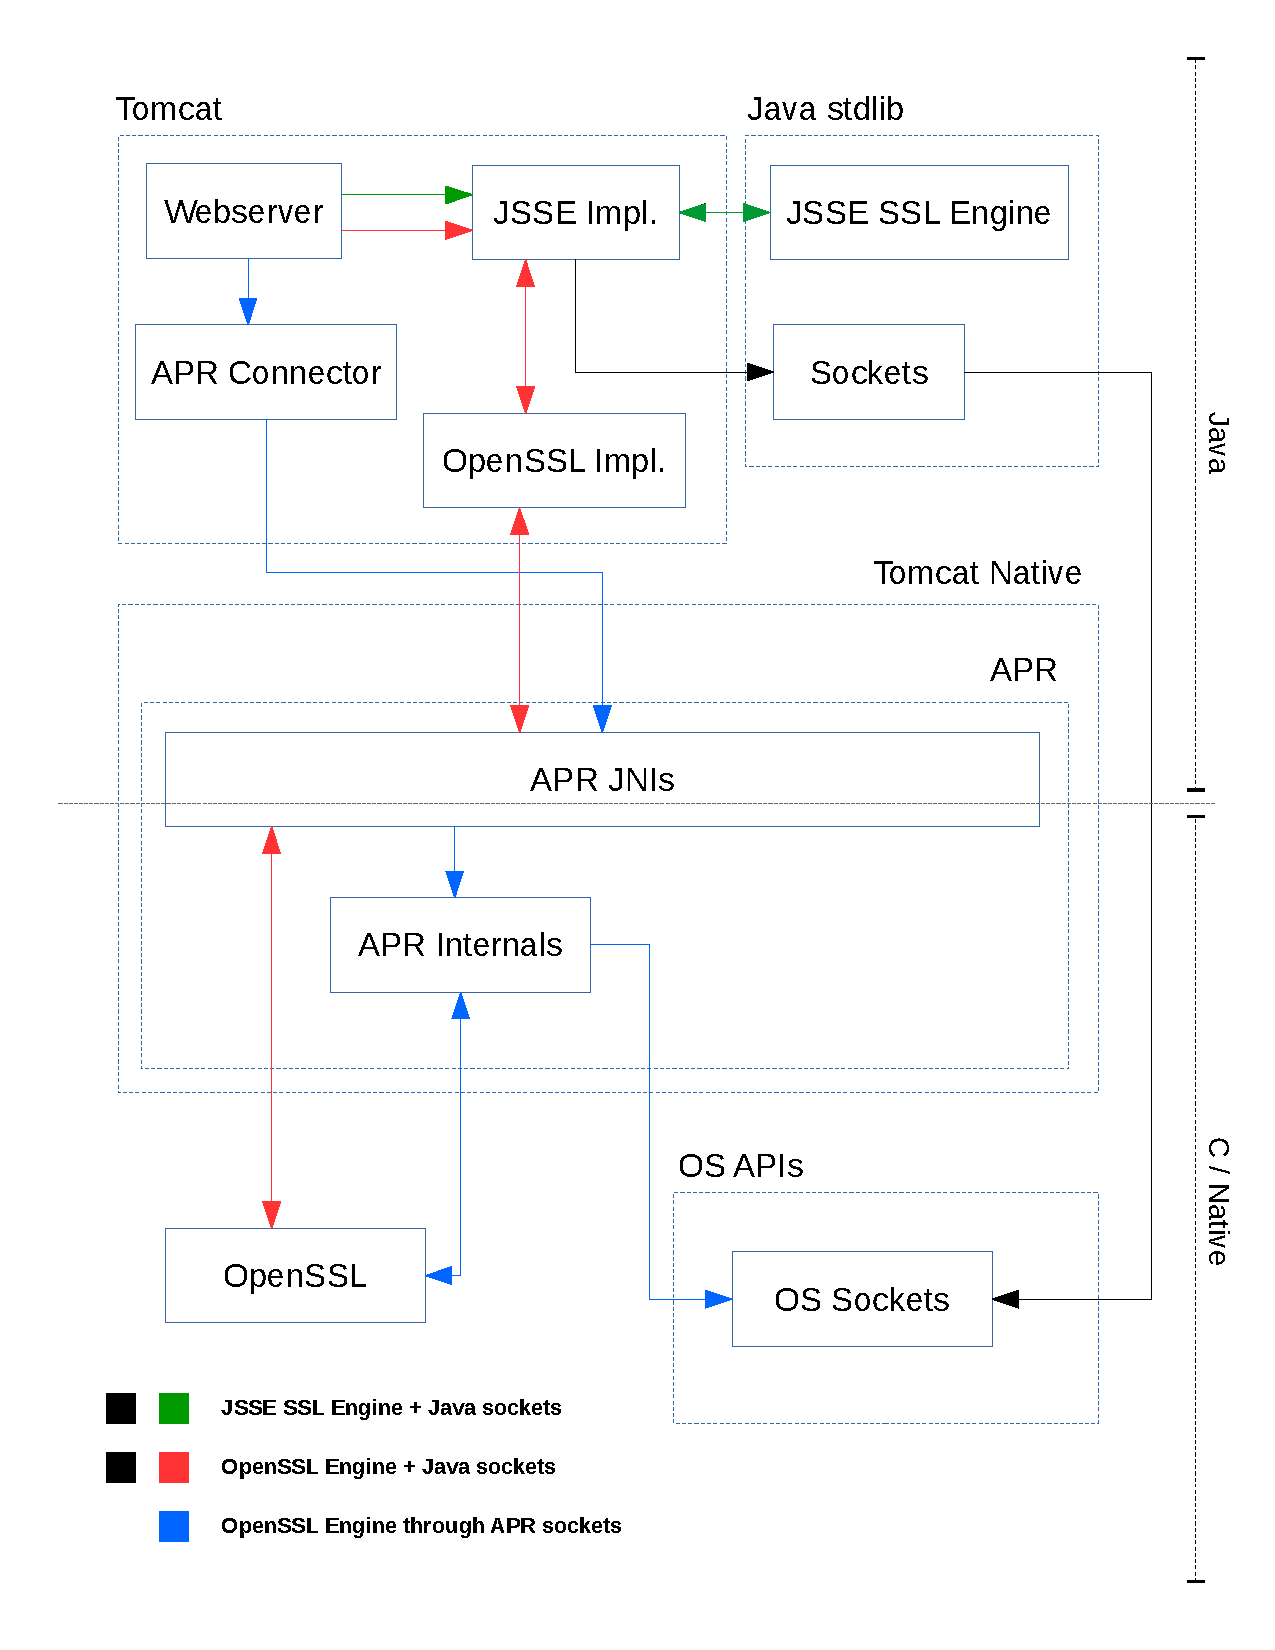
\includegraphics[scale=0.7]{diagram_current_way.pdf}
	\end{center}
	\caption{\textbf{Diagram showing the different ways to use TLS/SSL in Tomcat.}}
	\label{fig:current}
\end{figure}

\begin{figure}[!h]
	\begin{center}
		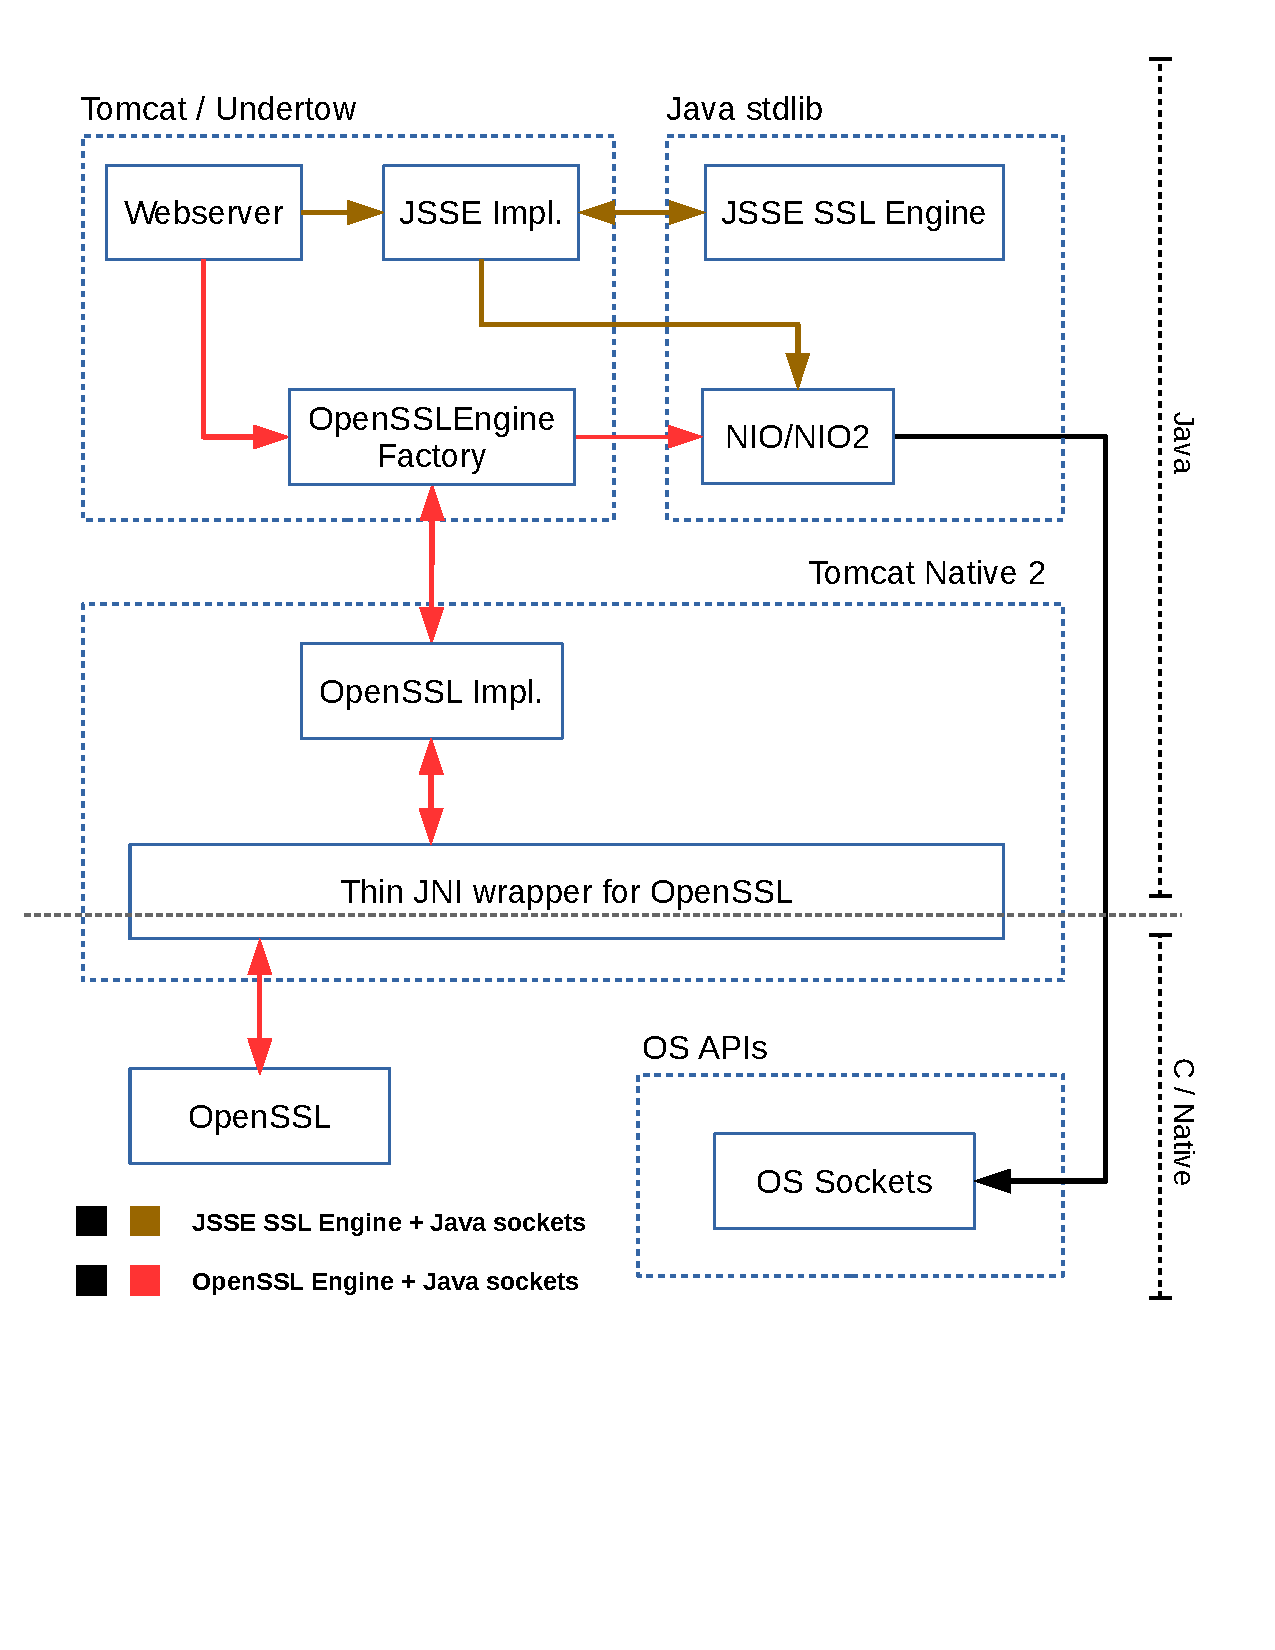
\includegraphics[scale=0.7]{diagram_goal.pdf}
	\end{center}
	\caption{\textbf{Diagram showing the end result of our project.}}
	\label{fig:goal}
\end{figure}

\FloatBarrier

\end{document}